\documentclass[12pt,a4paper]{article}
\usepackage[utf8]{inputenc}
\usepackage{amsmath}
\usepackage{amsfonts}
\usepackage{amssymb}
\usepackage{graphicx}
\begin{document}
\begin{center}
  \Large Assignment 2\\
  \large Distributed Algorithms
\end{center}
\begin{flushright}
  \begin{tabular}{ll}
    \textbf{Group 11} \\
    Dan Drewes     	  \\ 
    Manuela Hopp       \\ 
    John Mercouris    \\
    Malte Siemers     \\
  \end{tabular} 
\end{flushright}

\subsection*{Exercise 2.1: Election}
\paragraph*{a)} % Derive the time complexity of the Hirschberg-Sinclair election algorithm in the unite time complexity model! You can assume that all nodes initiate the algorithm at time t0 = 0.
There are $1+\lceil\log_2n\rceil$ phases.\newline
\newline
Best case topology:\newline We have $n = 2^k$ nodes. Thus there are $1+\log_2n$ phases. The messages sent out by different active nodes can be processed in parallel and in phase $i$ every active node sends out at most $4\cdot2^i$ messages of which half again can be processed in parallel because they are sent in opposite directions. Therefore worst case unit time complexity is $\sum\limits_{i=0}^{1+\log_2n-1}2 \cdot 2^{i} =2 \cdot \sum\limits_{i=0}^{\log_2n} 2^{i}=2 \cdot (2^{\log_2n+1}-1)=2 \cdot (2^{\log_2n} \cdot 2-1)=4 \cdot 2^{\log_2n}-2=4 \cdot n-2$ in total. Here we use $\sum\limits_{k=0}^{n} 2^{i}=2^{n+1}-1$ which can be proved by induction.\newline
\newline
Worst case topology:\newline Now we have $n=2^k+1$ nodes. Hence there are $1+\log_2(n-1)+1$ phases. Similar to the best case at most $2\cdot2^{i}$ messages have to be processed sequentially in phase $i$ except the last phase where there are $2n$ messages sent. It follows that $(\sum\limits_{i=0}^{\log_2(n-1)+1}2 \cdot 2^{i}) + 2n = 2 \cdot (\sum\limits_{i=0}^{\log_2(n-1)+1} 2^{i})+2n = 2 \cdot (2^{\log_2(n-1)+1}-1) + 2n = 2 \cdot (2^{\log_2(n-1)} \cdot 2-1) + 2n = 4 \cdot 2^{\log_2(n-1)}-2 +2n = 4 \cdot (n-1) -2 +2n = 6n-6$ is the worst case unit time complexity.
\paragraph{c)} % Implement the 3-phase election algorithm on trees (see lecture) and test your implementation using different tree topologies. Consider also the case that leaves are initiators. What is necessary to guarantee the proper execution of the algorithm? Give a reasonable answer.
\paragraph{d)} % Test your implementation of the 3-phase election algorithm on a non-tree topology, e.g., a hypercube or a ring. Does the algorithm still work properly? Give a reasonable answer.

\subsection*{Exercise 2.2: Termination}
\paragraph*{a)} % The algorithm for distributed termination detection presented in the paper R.K. Arora, S.P. Rana and M.N. Gupta.: ”Distributed termination detection algorithm for distributed computations” is wrong. Provide a counterexample and mention the mistake in the algorithm’s proof of correctness provided in the paper. Hint: The paper can be accessed from http://dx.doi.org/10.1016/0020-0190(86)90072-4
\begin{figure}[h]
\centering
 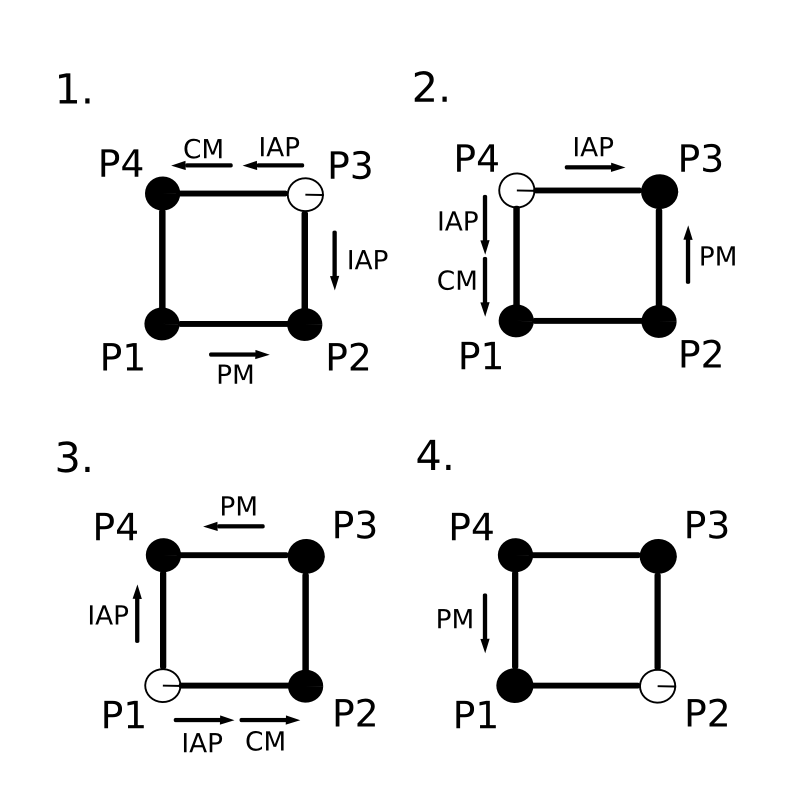
\includegraphics[width=0.6\textwidth]{2-2.png}
\end{figure}
In the figure above an example message sequence is pictured, that would lead to a false termination detection. Its valid for 4
and more nodes. P1 initiates a probe message (PM) after P2 and P4 went idle and informed P1 about that with an I-Am-Passive
message (IAP). Also, P3 sends a basic communication message (CM) to P4 that will set it to active and afterwards goes idle,
informing its neighbors about it (1.). As long as P2 is informed early enough, it will forward the PM. This sequence can be
repeated until P1 receives its own PM and starts the termination phase with P2 still being active (2. - 4.). Active nodes can
'travel' in front of a PM in this manner and a false termination is detected. \\
The error in the proof of correctnes is therefore in the last part, where they assume that a process that communicates with
another one that already forwarded a PM must purge this PM later. But as discribed above, thats not the case.
\paragraph{b)}
In the atom model actions on nodes are finished instantaneously. So the only time, that is consumed by an algorithm in the atom
model is the time, messages take between nodes. If a message was sent and recieced, it means that the action related to this
message is already finished. This also means, that if there is no messages on the way between nodes, the algorithm must have
terminated. With all messages having globally unique ids a control wave returning the same sets of sent (S) and received (R)
message ids proves, that no messages are on their way and so the algorithm is terminated.
\end{document}
